\section{Auswertung}
\label{sec:Auswertung}

\subsection{Bestimmung der mittleren Reichweite und Energie von Alpha-Teilchen}
\label{sub:Reichweite}

Zur Berechnung der mittleren Reichweite der $\alpha$-Teilchen wird der Versuch nach \autoref{sec:Durchführung} 
mit einem Abstand $x_0= \qty{1.7}{\centi\meter}$ durchgeführt und die Ergebnisse
in \autoref{tab:Zerfall1} aufgelistet.
Aus den Messwerten wird der effektive Abstand $x$ mithilfe von \autoref{eqn:x} berechnet und auch in \autoref{tab:Zerfall1} eingetragen.
Die Energie wird dadurch bestimmt, dass die Position des Maximums bei $p=\qty{0}{\milli\bar}$, nachfolgend als $N_0$ bezeichnet, dem
Energiewert $\SI{4}{\mega\eV}$ entspricht und die restlichen Channel und Energien
proportional dazu sind. Auch die Energiewerte werden in der Tabelle notiert.
Dieselbe Messung wird für einen Abstand von $x_0= \qty{3.0}{\centi\meter}$ wiederholt und die Ergebnisse analog zur ersten Messreihe 
in \autoref{tab:Zerfall2} notiert.

\begin{table}[H]
  \centering
  \caption{Messdaten zum Alpha-Zerfall bei einem Abstand von $x_0=1,7 cm.$}
  \label{tab:Zerfall1}
  \sisetup{table-format=1.2}
  \begin{tabular}{S[table-format=4.0] S[table-format=6.0] S[table-format=4.0] S S}
  \toprule
  \multicolumn{1}{p{2cm}}{Luftdruck $ p / \si{\milli\bar}$} &\multicolumn{1}{p{2cm}} {Anzahl $N$ der Intensitätsmaxima} & \multicolumn{1}{p{2cm}}{Kanal des Energiemaximums} &\multicolumn{1}{p{2cm}} {effektiver Abstand $x / \si{\centi\meter}$} &\multicolumn{1}{p{2cm}} {Energie $E / \si{\mega\eV}$}\\
  \midrule
    0    & 162524 & 1023  & 0     & 4.00 \\
    50   & 163290 & 960   & 0.08  & 3.75 \\
    100  & 163917 & 1039  & 0.17  & 4.06 \\
    150  & 165093 & 1023  & 0.25  & 4.00 \\
    200  & 165693 & 1023  & 0.34  & 4.00 \\
    250  & 164583 & 1023  & 0.42  & 4.00 \\
    300  & 166084 & 1023  & 0.50  & 4.00 \\
    350  & 170833 & 1039  & 0.59  & 4.06 \\
    400  & 169738 & 1023  & 0.67  & 4.00 \\
    450  & 170667 & 1007  & 0.76  & 3.94 \\
    500  & 170908 & 1023  & 0.84  & 4.00 \\
    550  & 170471 & 1023  & 0.92  & 4.00 \\
    600  & 170319 & 1023  & 1.01  & 4.00 \\
    650  & 169636 & 975   & 1.09  & 3.81 \\
    700  & 158958 & 911   & 1.17  & 3.56 \\
    750  & 158632 & 903   & 1.26  & 3.53 \\
    800  & 156749 & 879   & 1.34  & 3.44 \\
    850  & 153795 & 847   & 1.43  & 3.31 \\
    900  & 150817 & 847   & 1.51  & 3.31 \\
    950  & 147773 & 815   & 1.59  & 3.19 \\
    1000 & 144032 & 803   & 1.68  & 3.14 \\
  \bottomrule
  \end{tabular}
\end{table}
\begin{table}[H]
  \centering
  \caption{Messdaten zum Alpha-Zerfall bei einem Abstand von $x_0=3 cm.$}
  \label{tab:Zerfall2}
  \sisetup{table-format=2.2}
  \begin{tabular}{S[table-format=4.0] S[table-format=6.0] S[table-format=4.0] S S}
    \toprule
    \multicolumn{1}{p{2cm}}{Luftdruck $ p / \si{\milli\bar}$} &\multicolumn{1}{p{2cm}} {Anzahl $N$ der Intensitätsmaxima} & \multicolumn{1}{p{2cm}}{Kanal des Energiemaximums} &\multicolumn{1}{p{2cm}} {effektiver Abstand $x / \si{\centi\meter}$} &\multicolumn{1}{p{2cm}} {Energie $E / \si{\mega\eV}$}\\
    \midrule
    0    & 55548 & 1107 & 0.00 & 4.00\\
    50   & 54994 & 1023 & 0.15 & 3.70 \\
    100  & 54486 & 1023 & 0.30 & 3.70 \\
    150  & 54186 & 987  & 0.44 & 3.57 \\
    200  & 53546 & 911  & 0.59 & 3.29 \\
    250  & 52861 & 911  & 0.74 & 3.29 \\
    300  & 52766 & 896  & 0.89 & 3.24 \\
    350  & 51527 & 896  & 1.04 & 3.24 \\
    400  & 50461 & 847  & 1.18 & 3.06 \\
    450  & 48665 & 847  & 1.33 & 3.06 \\
    500  & 45128 & 847  & 1.48 & 3.06 \\
    550  & 40047 & 751  & 1.63 & 2.71 \\
    600  & 42233 & 719  & 1.78 & 2.60 \\
    650  & 44238 & 655  & 1.92 & 2.37 \\
    700  & 33459 & 652  & 2.07 & 2.36 \\
    750  & 7126  & 688  & 2.22 & 2.49 \\
    800  & 1878  & 687  & 2.37 & 2.48 \\
    850  & 195   & 687  & 2.52 & 2.48 \\
    900  & 67    & 686  & 2.67 & 2.48 \\
    950  & 28    & 686  & 2.81 & 2.48 \\
    1000 & 23    & 686  & 2.96 & 2.48 \\
  \bottomrule
  \end{tabular}
\end{table}

Zur Bestimmung der Reichweite der $\alpha$-Teilchen sind in \autoref{fig:plot1} und \autoref{fig:plot2} die Messwerte der Anzahl $N$ der Intensitätsmaxima
gegen den effektiven Abstand $x$ aufgetragen.
\begin{figure}[H]
\begin{subfigure}{\textwidth}
  \centering
  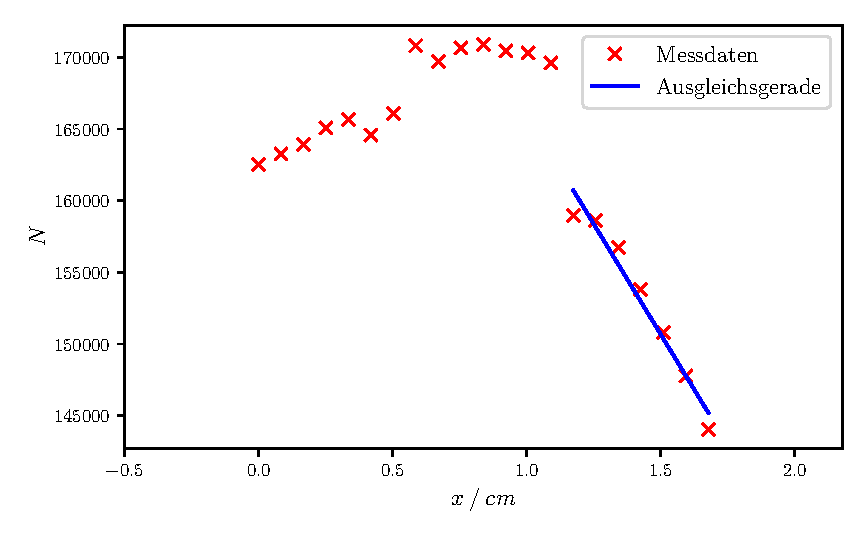
\includegraphics[scale=0.75]{build/plot1.pdf}
  \caption {Messdaten zur Bestimmung der mittleren Reichweite aus der Zählrate (Messreihe 1).}
  \label{fig:plot1}
\end{subfigure}
\hfill
\begin{subfigure}{\textwidth}
  \centering
  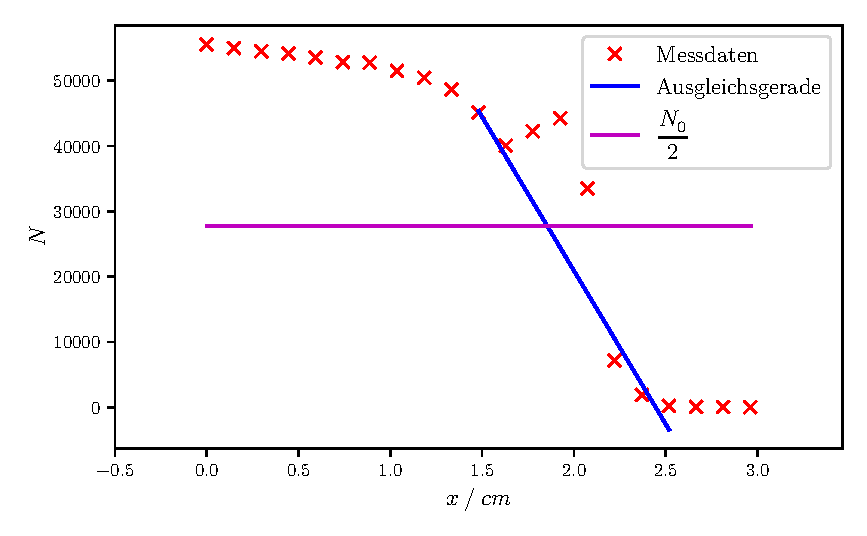
\includegraphics[scale=0.75]{build/plot2.pdf}
  \caption {Messdaten zur Bestimmung der mittleren Reichweite aus der Zählrate (Messreihe 2).}
  \label{fig:plot2}
\end{subfigure}
  \caption {Messdaten zur Bestimmung der mittleren Reichweite aus der Zählrate.}
\end{figure}

In \autoref{fig:plot1} wird eine lineare Regression der abfallenden Werte im Intervall $x=\qty{1.17}{\centi\meter}$ bis $x=\qty{1.68}{\centi\meter}$
mittels des Pythonmoduls matplotlib \cite{matplotlib} in der Form $N=m \cdot x +b$ durchgeführt.
Für die lineare Regression in \autoref{fig:plot2} geht das Intervall von $x=\qty{1.48}{\centi\meter}$ bis $x=\qty{2.37}{\centi\meter}$, jedoch 
werden hier die Werte zwischen $x=\qty{1.78}{\centi\meter}$ bis $x=\qty{2.07}{\centi\meter}$ nicht mit berücksichtigt, da diese nicht dem
linearen Verlauf folgen.
Die Parameter betragen hierbei
\begin{align*}
m_1 =& (-30827.55 ± 2675.73) \si{\per\centi\meter},\\
b_1 =& 196939.29 ± 3843.14\\
\shortintertext{und}
m_2 =& (-47049.01 ± 3437.24) \si{\per\centi\meter},\\
b_2 =& 115016.41 ± 7165.45.
\end{align*}

Eine horizontale Gerade ist außerdem auf Höhe von $\frac{N_0}{2}$ eingezeichnet. (Bei \autoref{fig:plot1} nicht im angezeigten Bereich.)
Der Schnittpunkt der beiden Geraden wird durch
\begin{align*}
  \frac{N_0}{2} &= m \cdot x + b \\
  x &= \frac{1}{m} \biggl(\frac{N_0}{2} - b \biggr) \\
\end{align*}
berechnet, wobei das errechnete $x$ der mittleren Reichweite $R_m$ der $\alpha$-Teilchen entspricht.
Da $m$ und $b$, fehlerbehaftete Größen sind, muss der Fehler von $R_m$ mithilfe der Gauß'schen Fehlerfortpflanzung
\begin{align*}
  \Delta R_m = \sqrt{\biggl(-\frac{1}{m^2} \biggl( \frac{N_0}{2} - b \biggr)\biggr)^2 \cdot (\Delta m)^2 + \biggl(\frac{1}{m}\biggr)^2 \cdot (\Delta b)^2}
\end{align*}
berechnet werden.
Somit ergibt sich für die mittleren Reichweiten $R_m$ der $\alpha$-Strahlung
\begin{align*}
  R_{m1}=& (6.40 \pm 0.60)\si{\centi\meter}\\
  R_{m2}=& (2.43 \pm 0.23)\si{\centi\meter}.
\end{align*}

Aus den mittleren Reichweiten lassen sich durch Umstellen der \autoref{eqn:Energiereichweite} die zugehörigen Energien $E_{\alpha}$ zu
\begin{align*}
  E_{\alpha, m1}=& (1.62 \pm 0.10)\si{\mega\eV}\\
  E_{\alpha, m2}=& (0.85 \pm 0.05)\si{\mega\eV}
\end{align*}
berechnen.

Die Messwerte der Energie $E$ aus \autoref{tab:Zerfall1} und \autoref{tab:Zerfall2} werden zudem in \autoref{fig:plot3} und \autoref{fig:plot4}
jeweils gegen $x$ aufgetragen.

\begin{figure}[H]
  \centering
  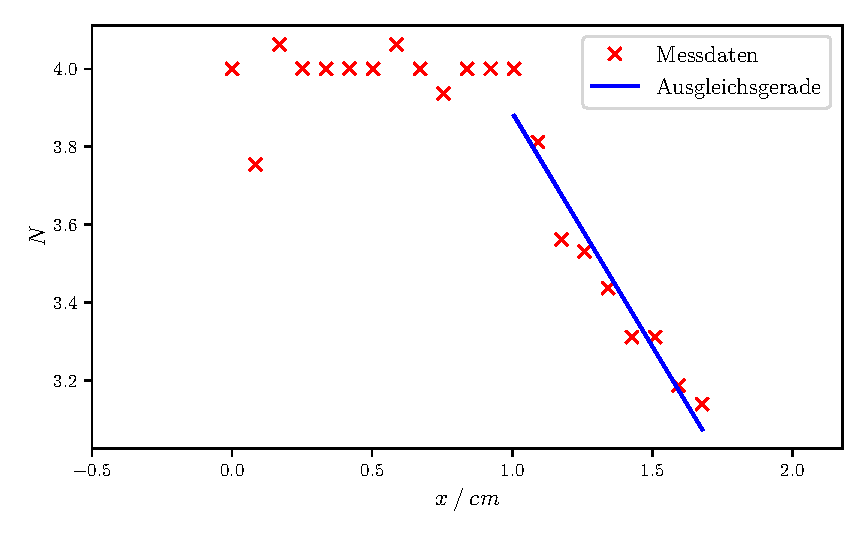
\includegraphics[width=\textwidth]{build/plot3.pdf}
  \caption {Bestimmung des Energieverlustes aus den Messdaten (Messreihe 1).}
  \label{fig:plot3}
\end{figure}

\begin{figure}[H]
  \centering
  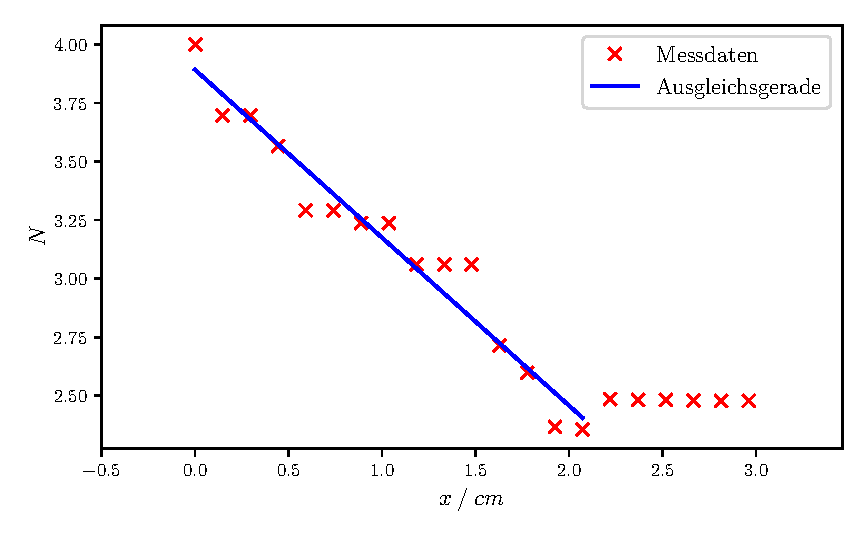
\includegraphics[width=\textwidth]{build/plot4.pdf}
  \caption {Bestimmung des Energieverlustes aus den Messdaten (Messreihe 2).}
  \label{fig:plot4}
\end{figure}

Auch hier werden Regressionsgeraden mittels Python erstellt und die Parameter der linearen Regressionen der Form
$E=c \cdot x +d $ lauten
\begin{align*}
  c =& (-1.199 \pm  0.120)\si{\mega\eV\per\centi\meter}\\
  d =& (5.087 \pm 0.164) \si{\mega\eV}\\
  c_2 =& (-0.717 \pm  0.044)\si{\mega\eV\per\centi\meter}\\
  d_2 =& (3.892 \pm 0.054) \si{\mega\eV}.
\end{align*}

Die Änderung der Energie ist die Steigung der Ausgleichsgerade. Somit ergeben sich für die Änderung der Energie $\frac{dE_\alpha}{dx}$
\begin{align*}
  \frac{dE_{\alpha, m1}}{dx} &= c = (-1.199 \pm  0.120)\si{\mega\eV\per\centi\meter}\\
  \frac{dE_{\alpha, m2}}{dx} &= c2 = (-0.717 \pm  0.044)\si{\mega\eV\per\centi\meter}.
\end{align*}



\subsection{Statistik des radioaktiven Zerfalls}
\label{sub:statistik}

Nach \autoref{sec:Durchführung} wird die Messung durchgeführt und die erhobenen Zählraten in \autoref{tab:stat}
notiert.
\begin{table}
  \centering
  \caption{100 statistische Messwerte der Zählrate bei $p = \SI{0}{\milli\bar}$ und Abstand $x = \SI{3.0}{\centi\meter}$.}
  \label{tab:stat}
  \sisetup{table-format=4.0}
  \begin{tabular}{S S S S S}
  \toprule
  4361 & 4256  &  4627 &  4272 &  4460 \\
  4104 &  4177 &  4266 &  4433 &  4389 \\
  4524 &  4259 &  4270 &  4630 &  4357 \\
  4638 &  4394 &  4602 &  4570 &  4528 \\ 
  4459 &  4436 &  4378 &  4466 &  4585 \\ 
  4564 &  4320 &  4455 &  4617 &  4347 \\ 
  4570 &  4305 &  4514 &  4534 &  4399 \\ 
  4384 &  4196 &  4525 &  4413 &  4573 \\  
  4379 &  4425 &  4290 &  4600 &  4153 \\  
  4580 &  4606 &  4265 &  4439 &  4370 \\  
  4529 &  4650 &  4506 &  4622 &  4488 \\  
  4415 &  4643 &  4491 &  4321 &  4629 \\  
  4379 &  4212 &  4080 &  4546 &  4298 \\  
  4345 &  4402 &  4607 &  4589 &  4706 \\  
  4539 &  4602 &  4371 &  4444 &  4173 \\  
  4586 &  4451 &  4576 &  4435 &  4577 \\  
  4419 &  4521 &  4455 &  4513 &  4483 \\  
  4321 &  4340 &  4289 &  4381 &  4348 \\  
  4580 &  4360 &  4560 &  4588 &  4723 \\  
  4313 &  4414 &  4216 &  4396 &  4651 \\  
  \bottomrule
  \end{tabular}
\end{table}


Aus den Daten in \autoref{tab:stat} werden zunächst der Mittelwert
\begin{align*}
  \mu &= \frac{1}{n} \sum_{i=1}^n N_i = 4443,47
\end{align*}
und die Standardabweichung
\begin{align*}
 \sigma &= \sqrt{ \frac{1}{n-1} \sum_{i=1}^n (N_i - \mu)^2  } =141,70 
\end{align*}
bestimmt.

\begin{figure}[H]
  \centering
  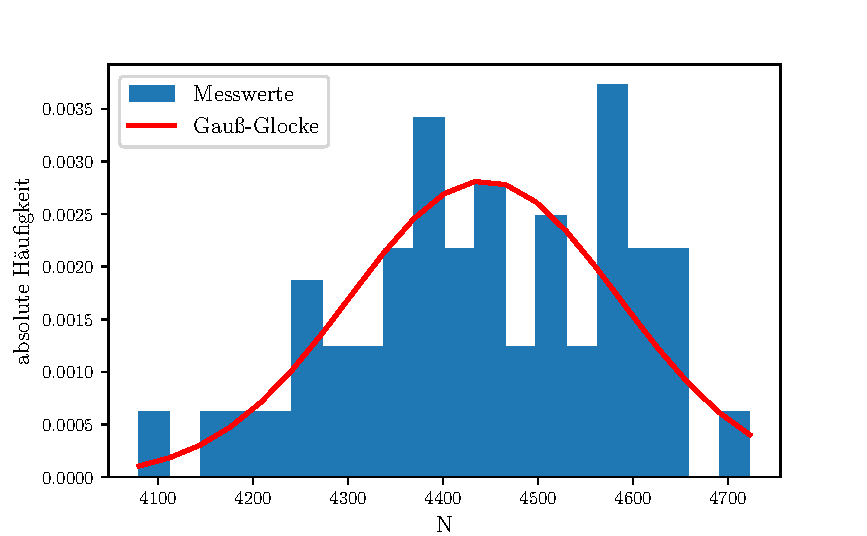
\includegraphics[width=\textwidth]{build/gauss.pdf}
  \caption {Gaußverteilung der Messwerte.}
  \label{fig:gauss}
\end{figure}

In \autoref{fig:gauss} sind die Werte gaußverteilt in einem Histogramm dargestellt. Die zugehörige Gaußkurve
\begin{align*}
  G(N, \mu, \sigma) = \frac{1}{\sigma \sqrt{2 \pi}} \cdot \text{exp} \left(- \frac{(N - \mu)^2}{2 \sigma^2} \right) \; .
\end{align*}
ist außerdem abgebildet.\\

Um die Poissonverteilung zu berechnen werden die Werte zuerst normiert
\begin{align*}
  M=N_\text{i, norm} = \frac{N_i - N_\text{min}}{n}.
\end{align*}
$N_\text{min}= 4080$ ist hierbei der kleinste der gemessenen Werte.
Die normierten Werte $M$ liegen nun zwischen $0$ und $7$.
Der Mittelwert der normalverteilten Werte beträgt
\begin{align*}
  \mu_P= 3.61.
\end{align*}

In \autoref{fig:poisson} sind nun die normalverteilten Messwerte und die theoretische Poissonverteilung nach der Formel
\begin{align*}
  p_{\mu_P}(M) =& \frac{\mu_P^M}{M!} \cdot \text{e}^{-\mu_P} 
\end{align*}
in einem Histogramm aufgetragen.


\begin{figure}[H]
  \centering
  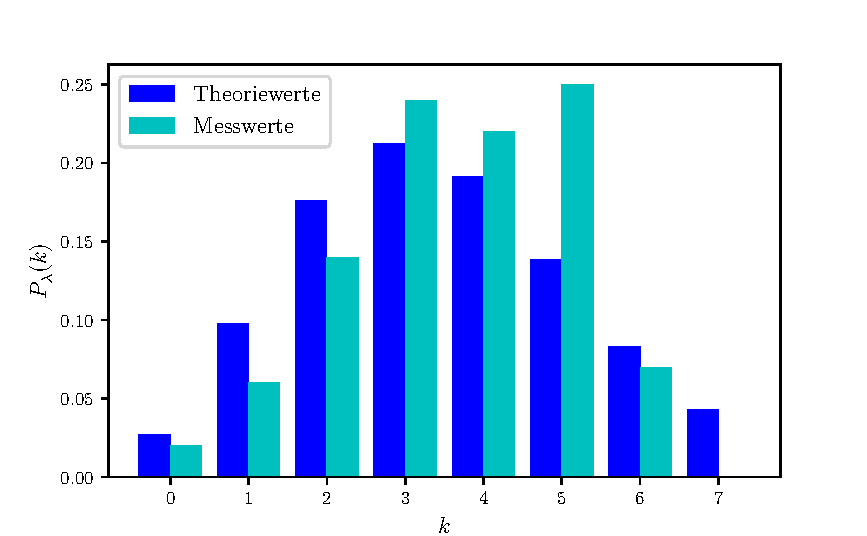
\includegraphics[width=\textwidth]{build/poisson.pdf}
  \caption {Poissonverteilung der Messwerte.}
  \label{fig:poisson}
\end{figure}


